\section{Terrain following advection of a stable thermal profile}
\label{sec:wobblyThetaAdvection}

This test is designed to investigate the cause of the potential temperature errors found in the gravity waves test.  The same potential temperature profile from the gravity waves test is advected over BTF and SnapCol grids using a terrain following velocity field that imitates a physical flow over orography.

\subsection{Specification}
The spatial domain, mountain profile and potential temperature profile are the same as those from the gravity waves test.  The potential temperature profile is fixed at the inlet and zero gradient at the outlet boundary so that it is advected consistently.  The upwind-biased advection scheme is used, as described in section~\ref{sec:method:discretisation}.  Following the gravity waves test, the model is integrated forward by 5 hours with a timestep $\Delta t = \SI{8}{\second}$. 

The velocity field is given by equation~\ref{eqn:wobblyTracerAdvection:velocity} but, because the mountain profile is different, the derivative of terrain height, $\partial h / \partial z$, is
\begin{align}
\frac{\partial h}{\partial x} &= - 2 h_0 \exp \left( - \left( \frac{x}{a} \right)^2 \right) \cos \left( \frac{\pi x}{\lambda} \right) \left[
\frac{\pi}{\lambda} \sin \left(\frac{\pi x}{\lambda} \right) +
\frac{x}{a^2} \cos \left( \frac{\pi x}{\lambda} \right) \right]
\end{align}

\subsection{Results}
Potential temperature anomalies after 5 hours on the BTF and SnapCol grids are shown in figure~\ref{fig:wobblyThetaAdvection:thetaDiff}.  On both grids, columns of lower potential temperature are seen above the mountain peaks, due to the orographic lifting of air at the ground.  Hence, the highest central peak produces the largest cold anomaly.  Similarly, on both grids, a warm anomaly is found near the outlet (not shown).  It is created by high potential temperature initially above the mountain peaks being advected down to the ground.

Similar to the gravity waves result, on the SnapCol grid, potential temperature anomalies are found near the ground in the lee of the mountain (see figure~\ref{fig:wobblyThetaAdvection:thetaDiff:snapCol}).  Importantly, however, the anomalies are reversed when compared to the result from the gravity waves test in figure~\ref{fig:gw:thetaDiff:snapCol}: in this advection test, the layer nearest the ground is anomalously cold and the layer above it is anomalously warm.

Vertical profiles of potential temperature on the BTF and SnapCol grids are presented in figure~\ref{fig:wobblyThetaAdvection:theta}, for comparison with the same profiles from the gravity waves test in figure~\ref{fig:gw:exner-theta}.
Differences in potential temperature from the initial profile are compared to the results from the gravity waves test in table~\ref{tab:theta-sample}.

Given that the potential temperature anomalies are inverted compared to the gravity waves test, it is not certain that the Lorenz computational mode is excited by advection errors, although this is still a possible cause.

It is important to note two differences between the gravity waves test and this advection test.  First, only the advection equation is being solved instead of the fully-compressible Euler equations that were solved in the gravity waves test.  Second, the velocity field that is prescribed does not match exactly the flow in the gravity waves test.  Improvements to the velocity field are proposed in section~\ref{sec:further-work:gw}.

\begin{figure}
	\captionsetup[subfigure]{position=b}
	\centering
	\subcaptionbox{BTF \label{fig:wobblyThetaAdvection:thetaDiff:btf}}[0.49\textwidth]{\includegraphics[height=2.6in,angle=270]{openfoam/cases/wobblyThetaAdvection/btf/schaerExp/cubicUpwindCPCFit/18000/thetaDiff.eps}}
	\hfill
	\subcaptionbox{SnapCol \label{fig:wobblyThetaAdvection:thetaDiff:snapCol}}[0.49\textwidth]{\includegraphics[height=2.6in,angle=270]{openfoam/cases/wobblyThetaAdvection/snapCol/schaerExp/cubicUpwindCPCFit/18000/thetaDiff.eps}}
	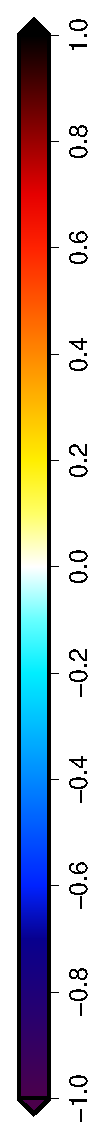
\includegraphics[height=5in,angle=270]{legends/thetaDiffWide.eps}
%
	\caption{Potential temperature anomalies of terrain following advection of a stable potential temperature profile at $t = \SI{18000}{\second}$.}
	\label{fig:wobblyThetaAdvection:thetaDiff}
\end{figure}
